% ==============================================================================
\subsection{Context}\label{aa:res:context}
\begin{figure}[h]
  \centering
  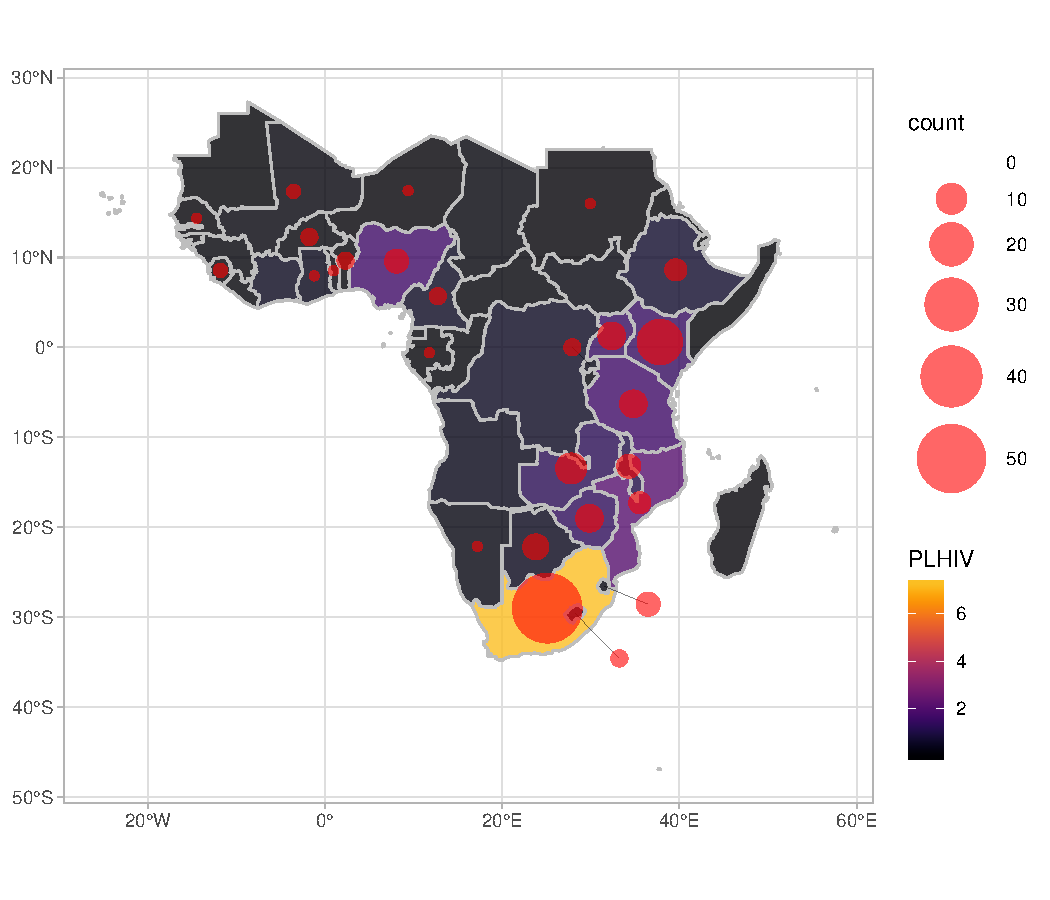
\includegraphics[width=0.8\linewidth]{map-n-vs-plhiv}
  \caption{Map showing number of articles (of \na total)
    applying HIV transmission modelling in each country vs
    the number of people living with HIV (PLHIV, millions)}
  \label{fig:map}
\end{figure}
% ==============================================================================
\subsection{Risk Heterogeneity}\label{aa:res:risk}
% ------------------------------------------------------------------------------
\subsubsection{Distributions}
\twocolumn
\filedef{\projectroot/out/tex/config/plot.list.dist}
\foreach \var/\title in \filedata{\hspace{0pt}%
  \begin{minipage}[t][.33\textheight][t]{\linewidth}
    \includegraphics[width=\linewidth]{{d.\var}.pdf}
    \captionof{figure}{\title}
    \label{fig:d:\var}
  \end{minipage}}
\onecolumn
\clearpage
% ==============================================================================
\subsection{ART Prevention Impact}\label{aa:res:api}
The following figures show the projected ART prevention impact (Dataset~B),
stratified by various factors of heterogeneity (colours).
The left panels show the relative reduction in HIV incidence rate;
the right panels show the relative reduction in cumulative new HIV infections;
both as compared to a base-case scenario reflecting status quo.
The number of articles (scenarios) reporting
incidence reduction, cumulative infections averted, both, or either was:
\x{n/n.a.api.inc}~(\x{n/n.s.api.inc}),
\x{n/n.a.api.chi}~(\x{n/n.s.api.chi}), 
\x{n/n.a.api.both}~(\x{n/n.s.api.both}), and
\x{n/n.a.api}~(\x{n/n.s.api}), respectively.
If any article included multiple scenarios of ART scale-up,
then each scenario was included separately,
but the size of each data point was reduced
in proportion to the number of scenarios;
so articles with only one scenario have the largest data points.
Some scenarios have multiple data points if multiple time horizons were reported.
If any factor could not be quantified due to missing data or varying values,
the data point is grey.
A small random offset has been added to the data points to reduce overlap.
\filedef{\projectroot/out/tex/config/plot.list.api}
\foreach \var/\title in \filedata{
  \begin{figure}[h]
    \begin{subfigure}{0.5\linewidth}
      \includegraphics[width=\linewidth]{{inc.s.\var}.pdf}
    \end{subfigure}%
    \begin{subfigure}{0.5\linewidth}
      \includegraphics[width=\linewidth]{{chi.s.\var}.pdf}
    \end{subfigure}
    \caption{\title}
    \label{fig:api:\var}
  \end{figure}
}
